\documentclass[11pt]{article}

\usepackage[margin=1in]{geometry}
\usepackage{amsmath}
\usepackage{graphicx}
\usepackage{booktabs}
\usepackage{longtable}
\usepackage{array}
\usepackage[hidelinks]{hyperref}
\usepackage{enumitem}
\usepackage{titlesec}
\usepackage{xcolor}
\usepackage{parskip}
\usepackage{graphicx}
\usepackage{csvsimple}

\graphicspath{ {../figs} }

\titleformat{\section}{\normalfont\Large\bfseries}{\thesection}{1em}{}
\titleformat{\subsection}{\normalfont\large\bfseries}{\thesubsection}{1em}{}

\newcommand{\placeholder}[1]{%
	\begin{center}
		\fbox{\parbox{0.9\textwidth}{\centering\itshape #1}}
	\end{center}
}

\title{\vspace{-1.5cm}CGS4144 Bioinformatics --- Assignment 2}
\author{}
\date{}

\begin{document}
	
	\maketitle
	\vspace{-2cm}
	
	\section*{Team}
	
	\begin{center}
		\begin{tabular}{|>{\raggedright}p{4.5cm}|>{\raggedright}p{5cm}|>{\raggedright\arraybackslash}p{4cm}|}
			\hline
			\textbf{Name} & \textbf{Email} & \textbf{GitHub} \\
			\hline
			Ethan Klasky & eklasky@ufl.edu & E53klasky \\
			\hline
			Amit Athi Kesavan & amit.athikesvan@ufl.edu & amitathik7 \\
			\hline
			Timothy Wang & timothy.wang@ufl.edu & timothyw8 \\
			\hline
		\end{tabular}
	\end{center}
	
	\vspace{0.5em}
	\noindent\textbf{Data:} \url{https://www.refine.bio/dataset/31f09143-bf06-4a05-adcf-6c9c0e1d892f}
	
	\noindent\textbf{Scientific Question:} Can gene expression patterns in blood distinguish tuberculosis patients who have different treatment outcomes?
	
	\noindent\textbf{GitHub Repository for Project:} \url{https://github.com/E53klasky/CGS4144}
	
	\section{Data Loading and Expression Variation}
	
	The SRP092402 expression matrix contained 43{,}363 genes across 909 samples. The original gene identifiers began with ENSG (e.g. ENSG00000000003) instead of gene names, so they were converted to their corresponding human gene names when a mapping was available. A total of 33{,}191 gene IDs were successfully converted, while IDs without an available mapping were retained as their original Ensembl identifiers. The expression data were log-transformed using $\log_2(x+1)$, and the median expression of each gene across all samples was calculated. The density plot below shows that most genes have low median expression, while a smaller number have much higher expression, producing a long tail toward higher expression values.
	
	\begin{figure}[h]
		\centering
		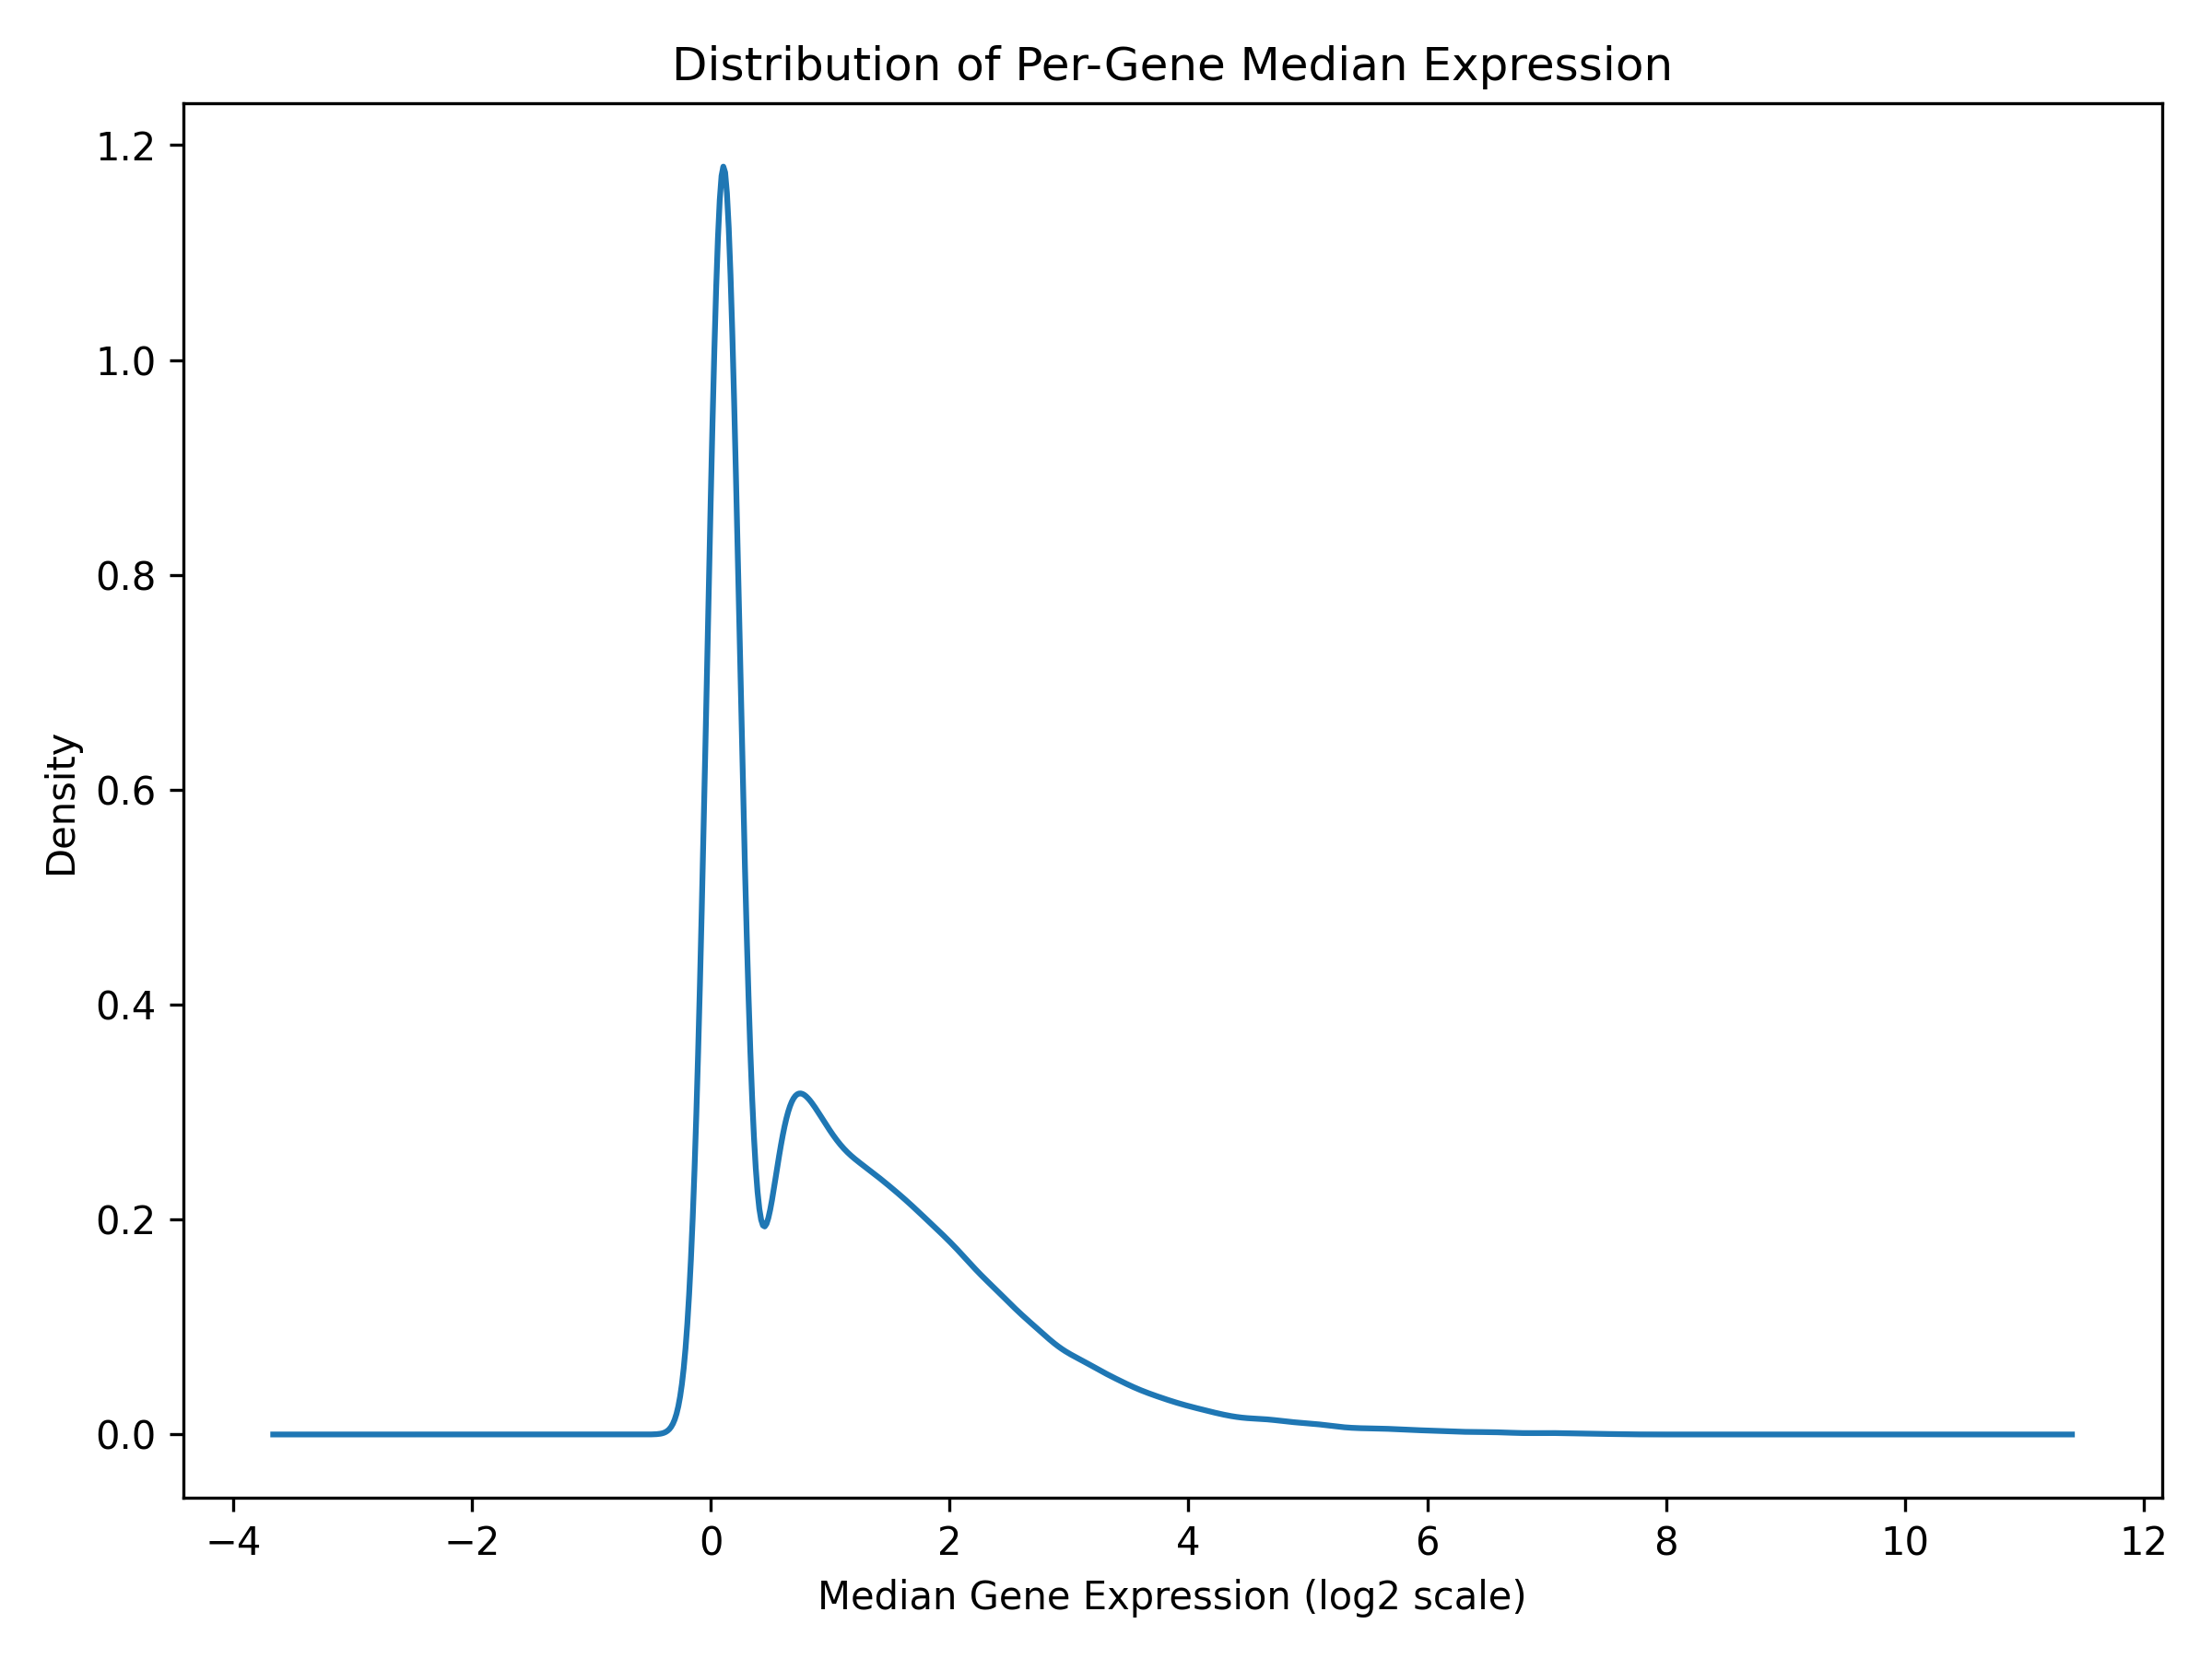
\includegraphics[scale=0.5]{gene_expression_density.png}
		\caption{Density plot of per-gene median expression (log2 scale).}
		\label{fig:density}
	\end{figure}
	
	\section{Dimensionality Reduction: PCA, t-SNE, and UMAP}
	
	PCA, t-SNE, and UMAP were used to visualize differences in gene expression between TB subjects and healthy controls. For the PCA plot, the expression data were $\log_2$-transformed and mean-centered prior to decomposition via SVD. PC1 and PC2 explained 7.3\% and 4.6\% of the total variance, respectively, and the two groups largely overlapped rather than forming distinct clusters. For the t-SNE plot, a perplexity of 20 was used; the plot also showed substantial overlap between groups, although some healthy-control samples formed small local groups. For the UMAP plot, 15 neighbors were used; UMAP showed the clearest local grouping of healthy controls, particularly on one side of the plot, but healthy and TB samples were still not completely separated.
	
	\begin{figure}[h]
		\centering
		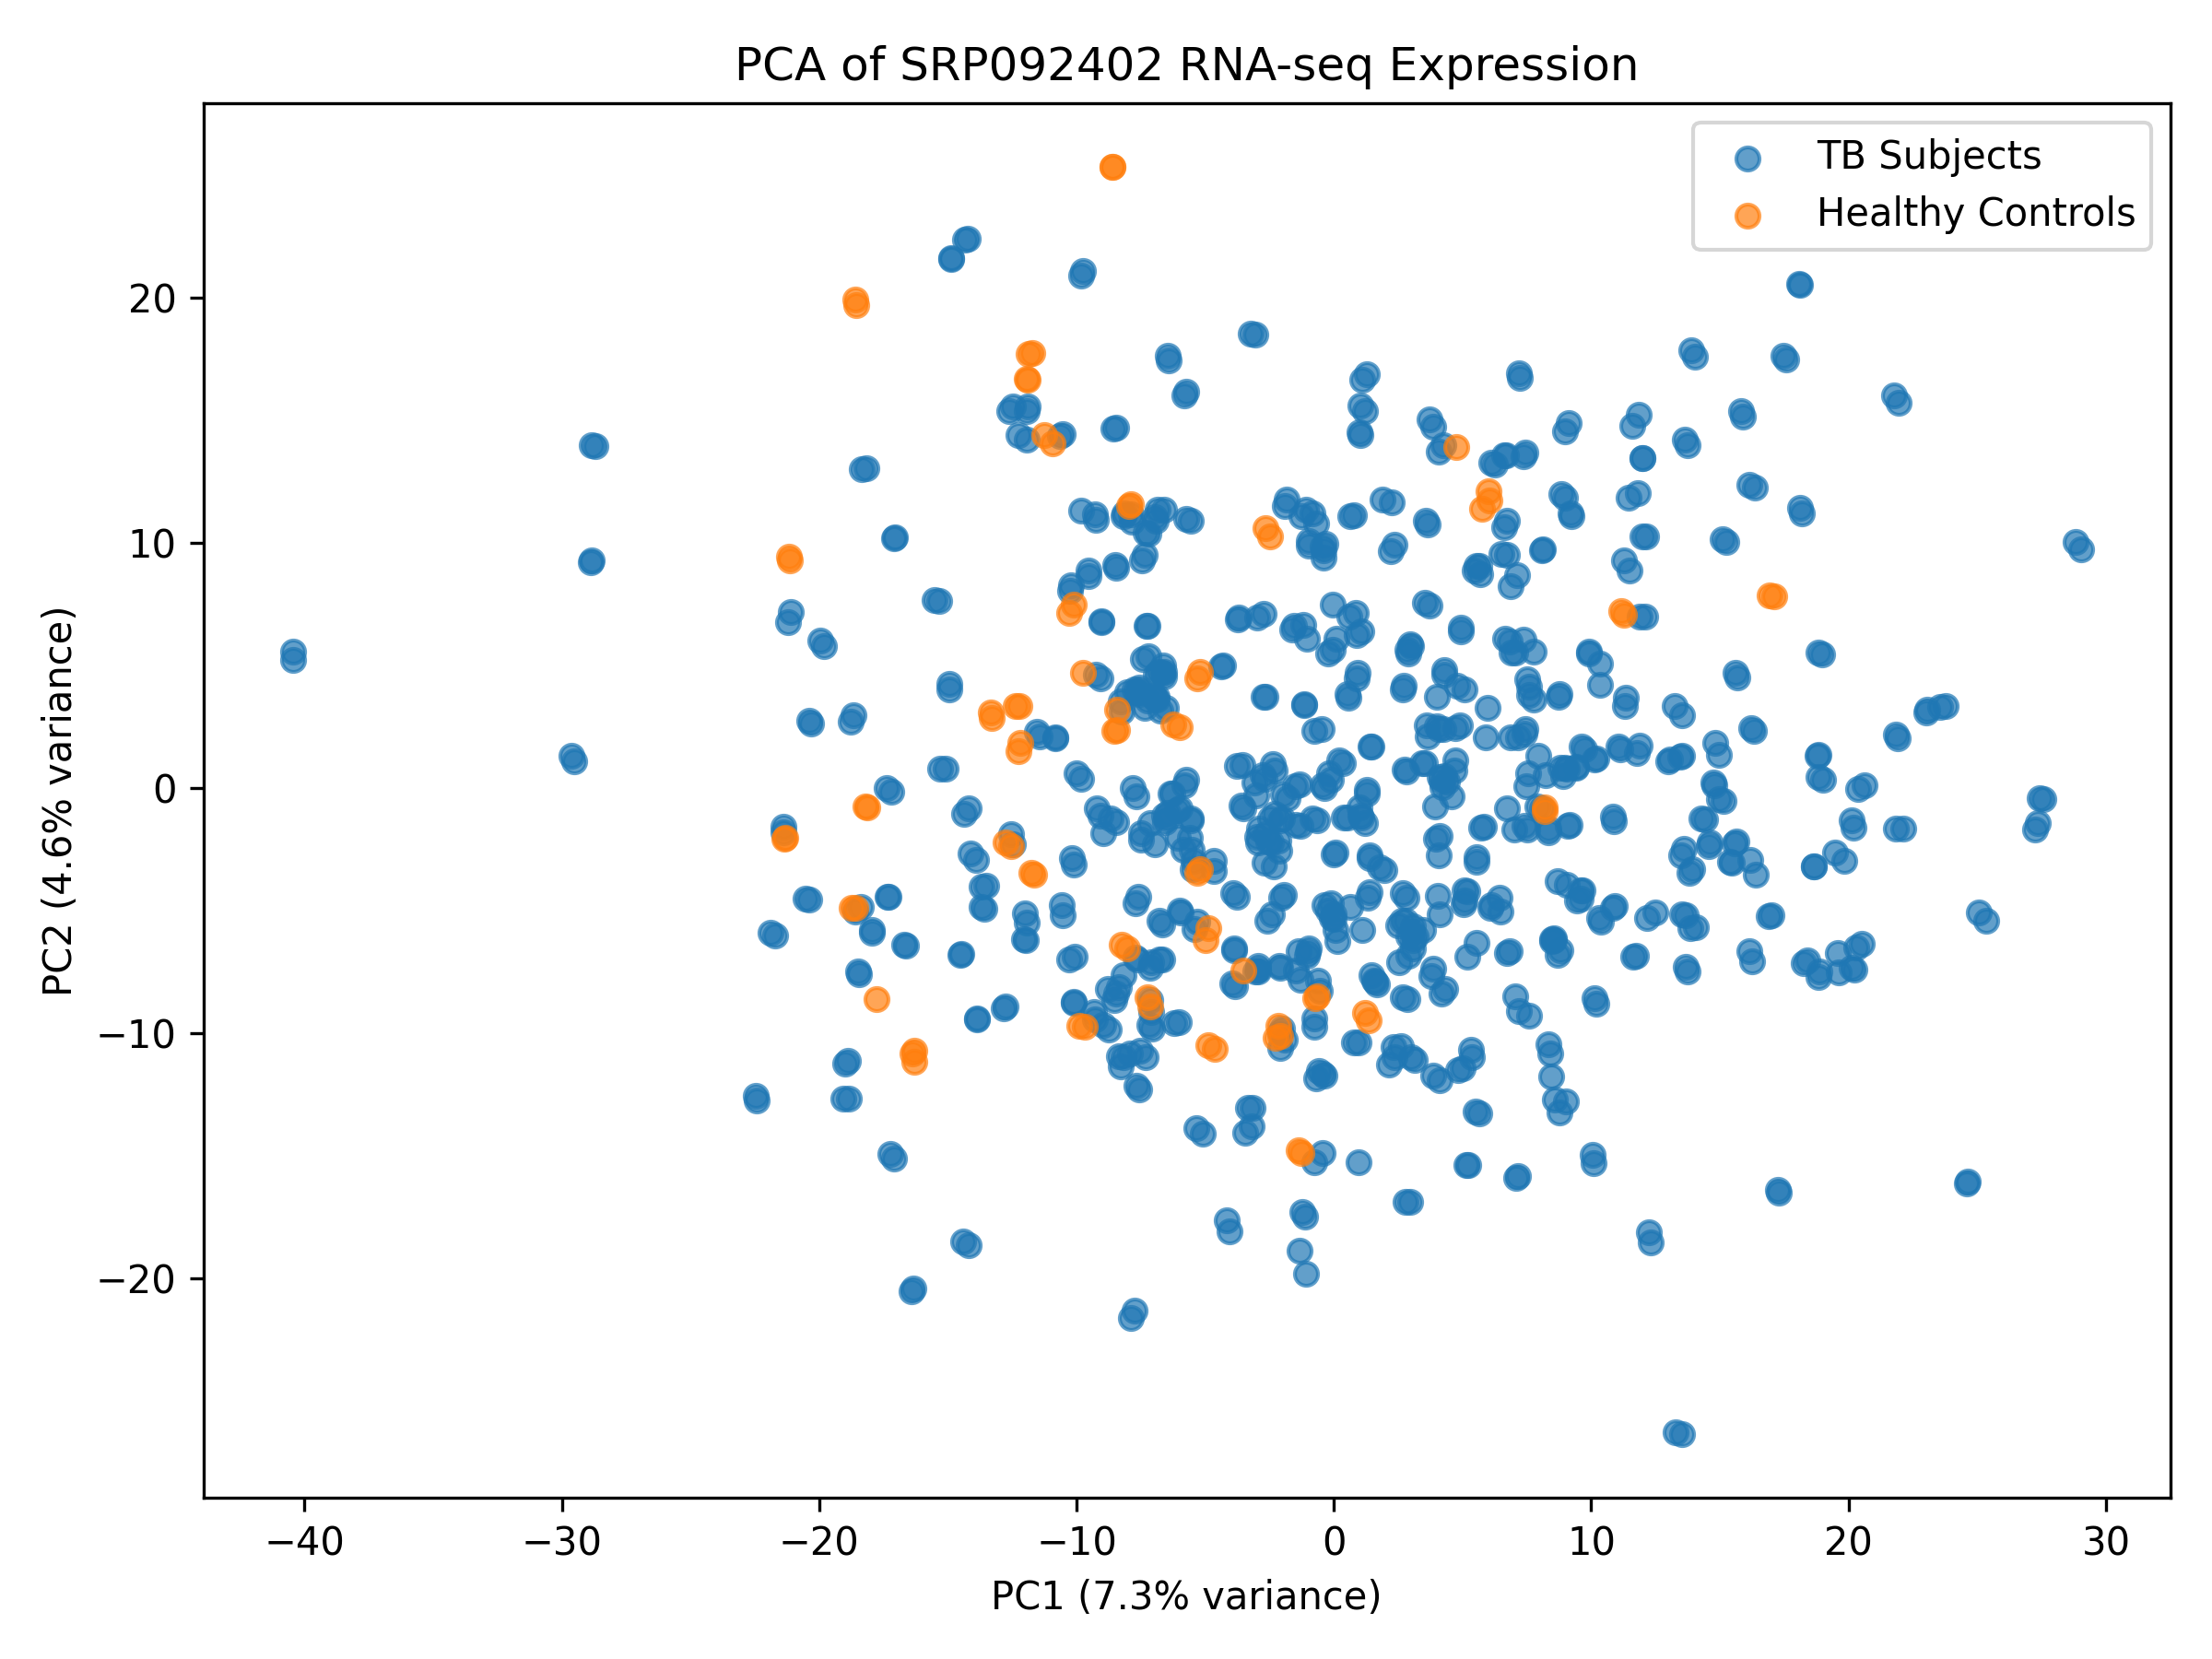
\includegraphics[scale=0.5]{PCA.png}
		\caption{PCA of TB subjects vs.\ healthy controls.}
		\label{fig:pca}
	\end{figure}
	
	\begin{figure}[h]
		\centering
		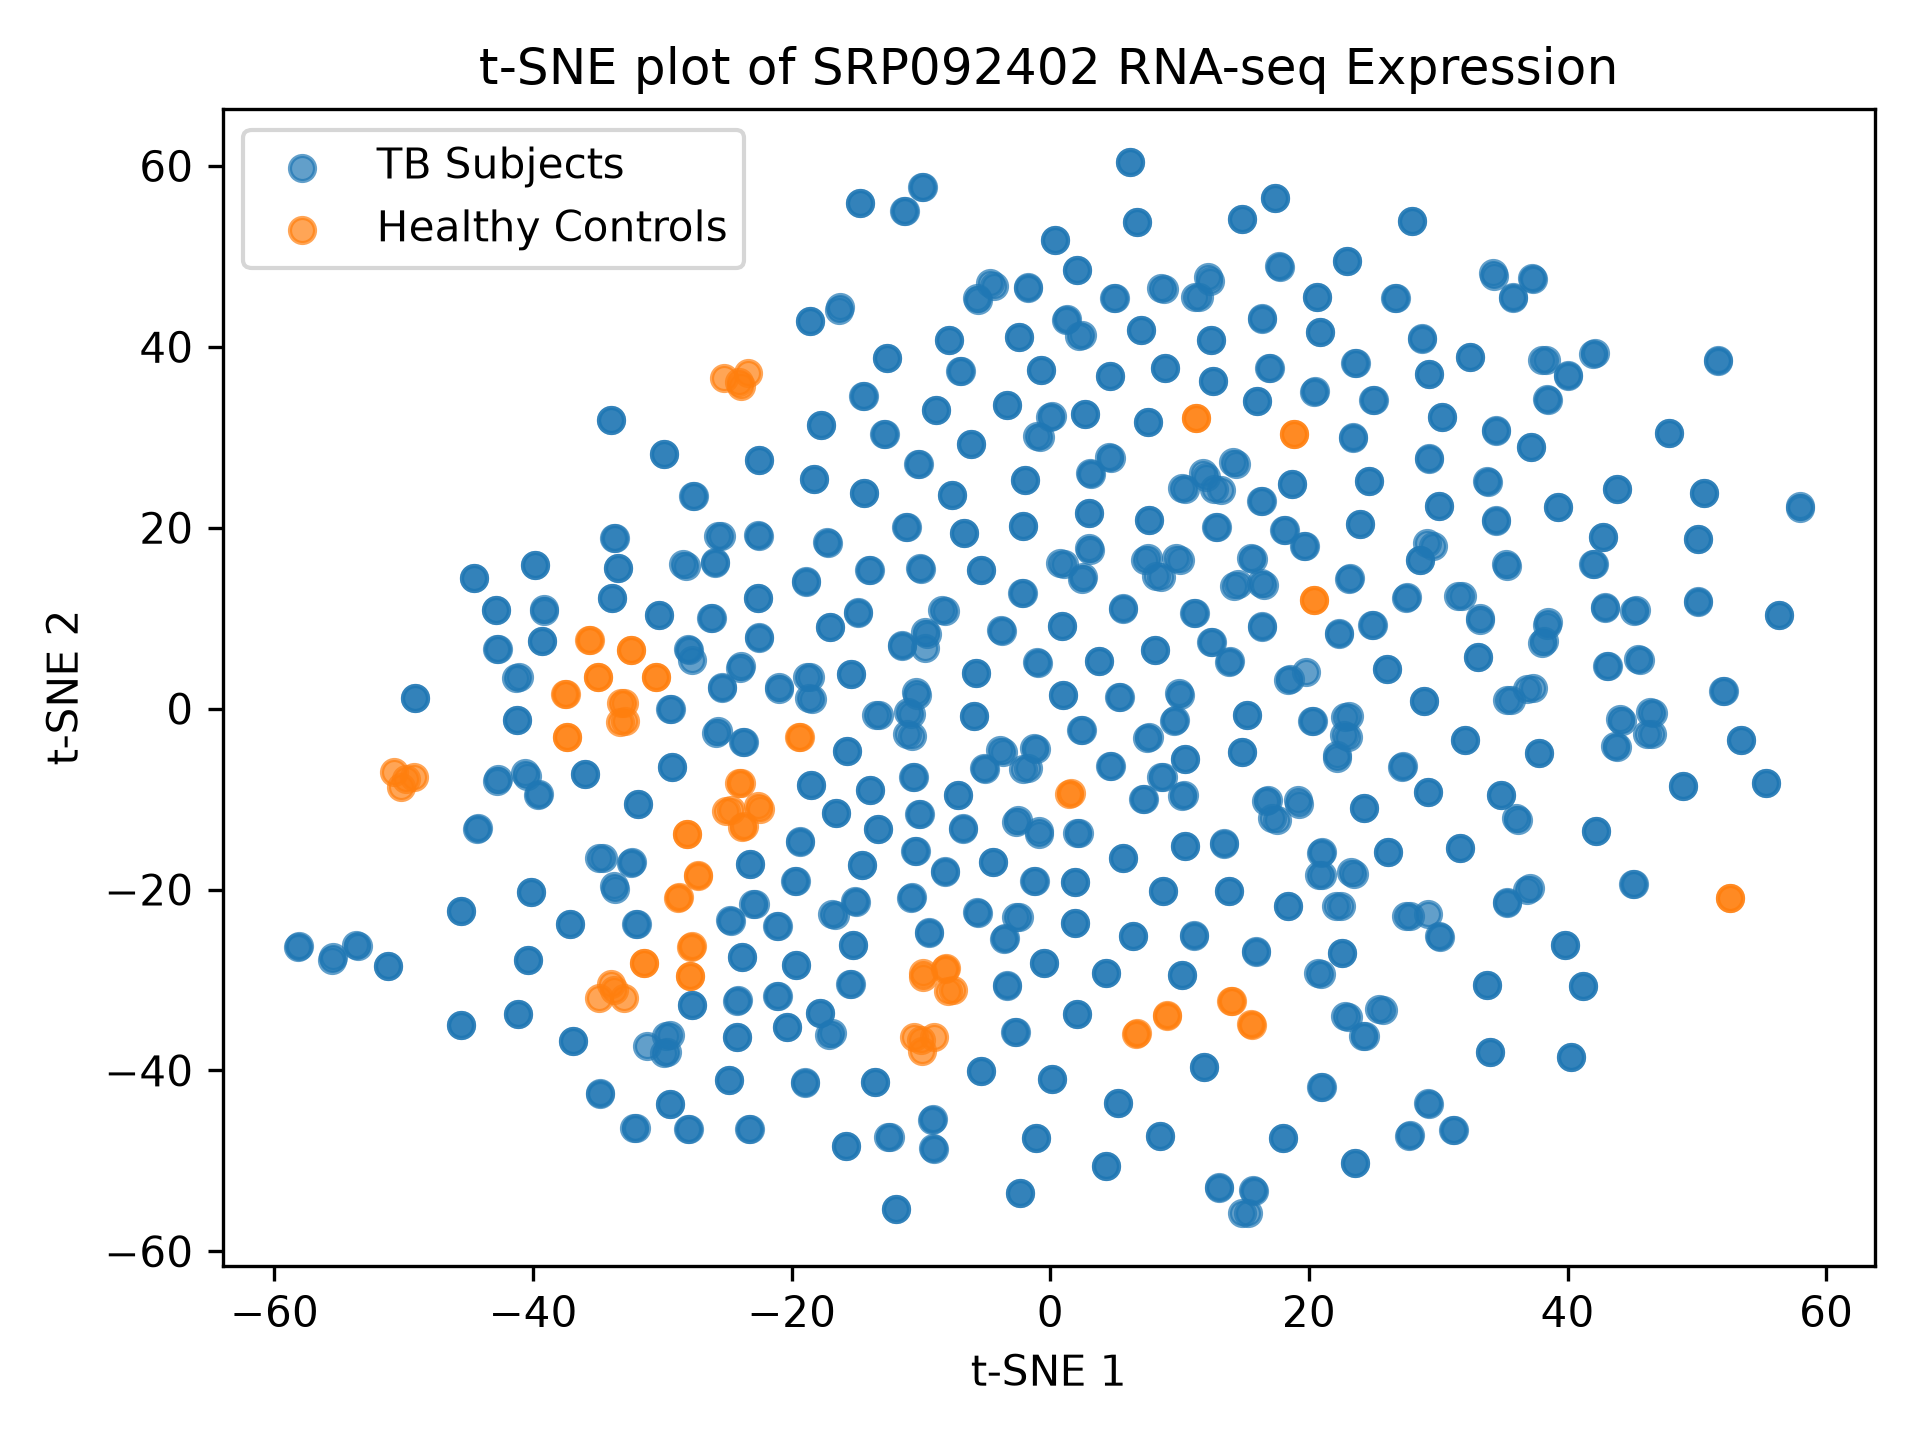
\includegraphics[scale=0.5]{t-SNE.png}
		\caption{t-SNE of TB subjects vs.\ healthy controls (perplexity = 20).}
		\label{fig:tsne}
	\end{figure}
	
	\begin{figure}[h]
		\centering
		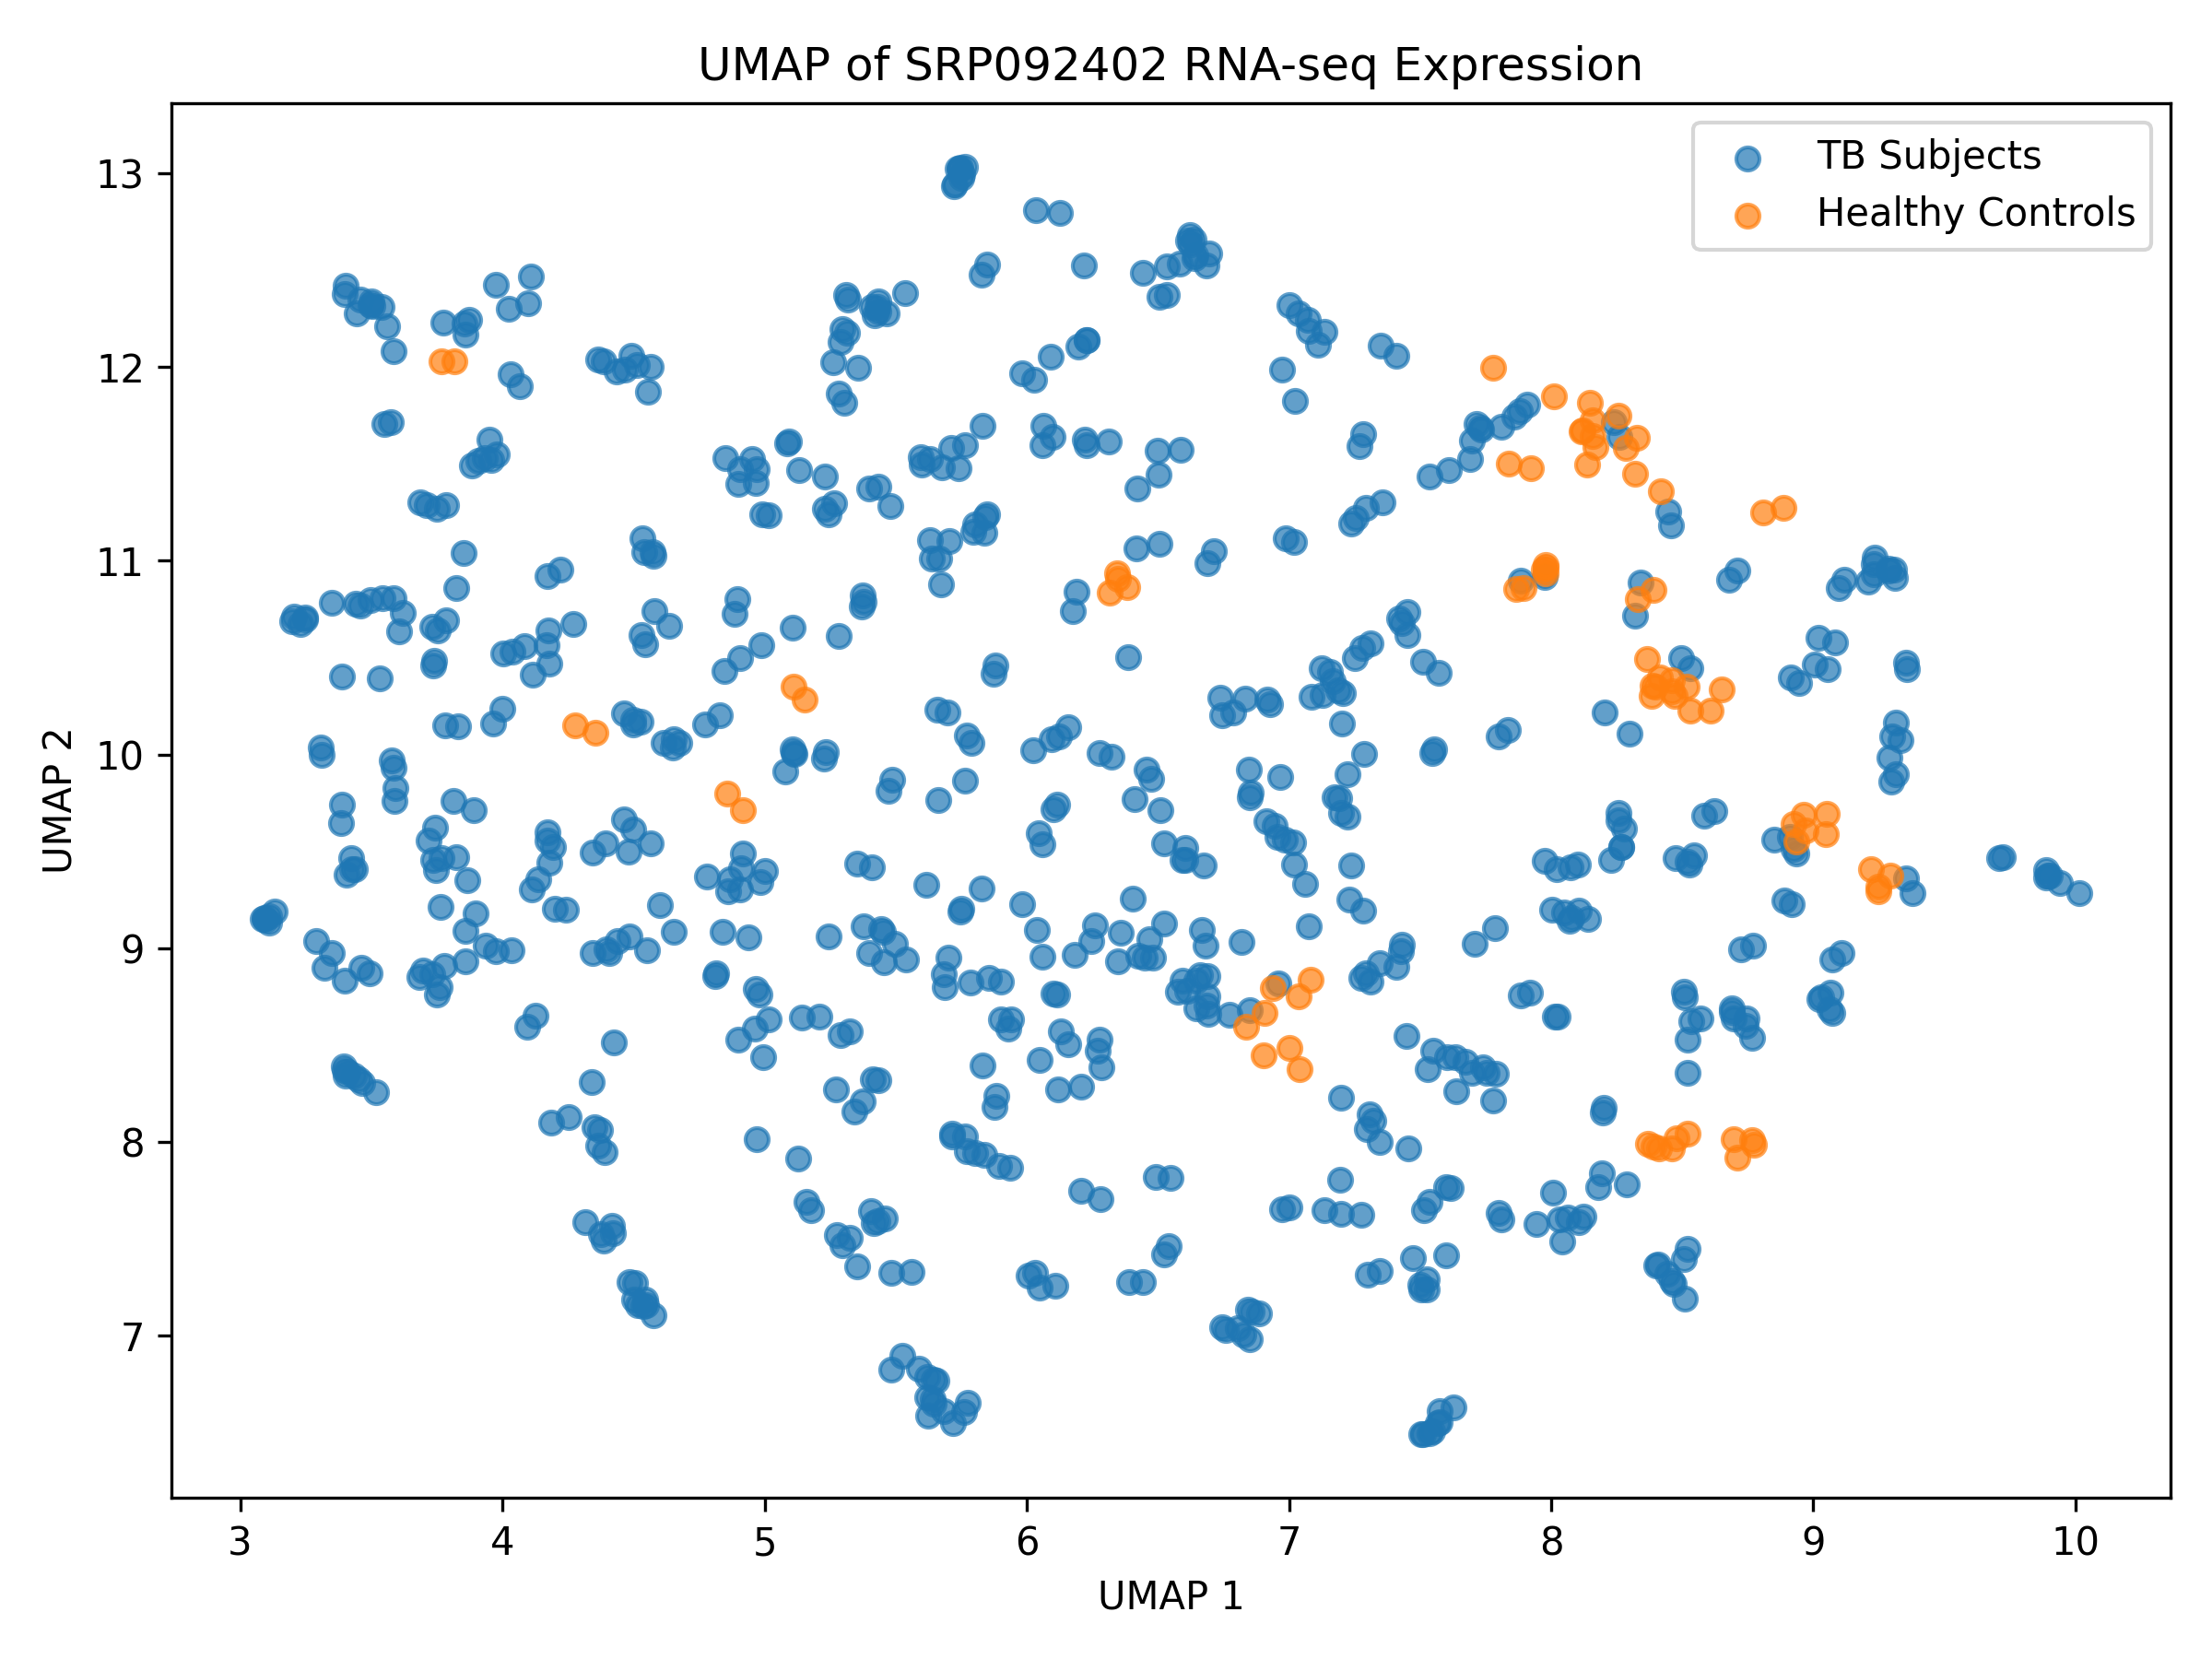
\includegraphics[scale=0.5]{UMAP.png}
		\caption{UMAP of TB subjects vs.\ healthy controls (n\_neighbors = 15).}
		\label{fig:umap}
	\end{figure}
	
	\section{Differential Expression Analysis}
	
	A Welch's two-sample $t$-test was performed independently on each gene to identify genes that were significantly differentially expressed between the TB and healthy-control groups, with Benjamini--Hochberg correction applied for multiple testing. The volcano plot below shows genes that were significantly more or less expressed in the TB group relative to the healthy-control group.
	
	\begin{figure}[h]
		\centering
		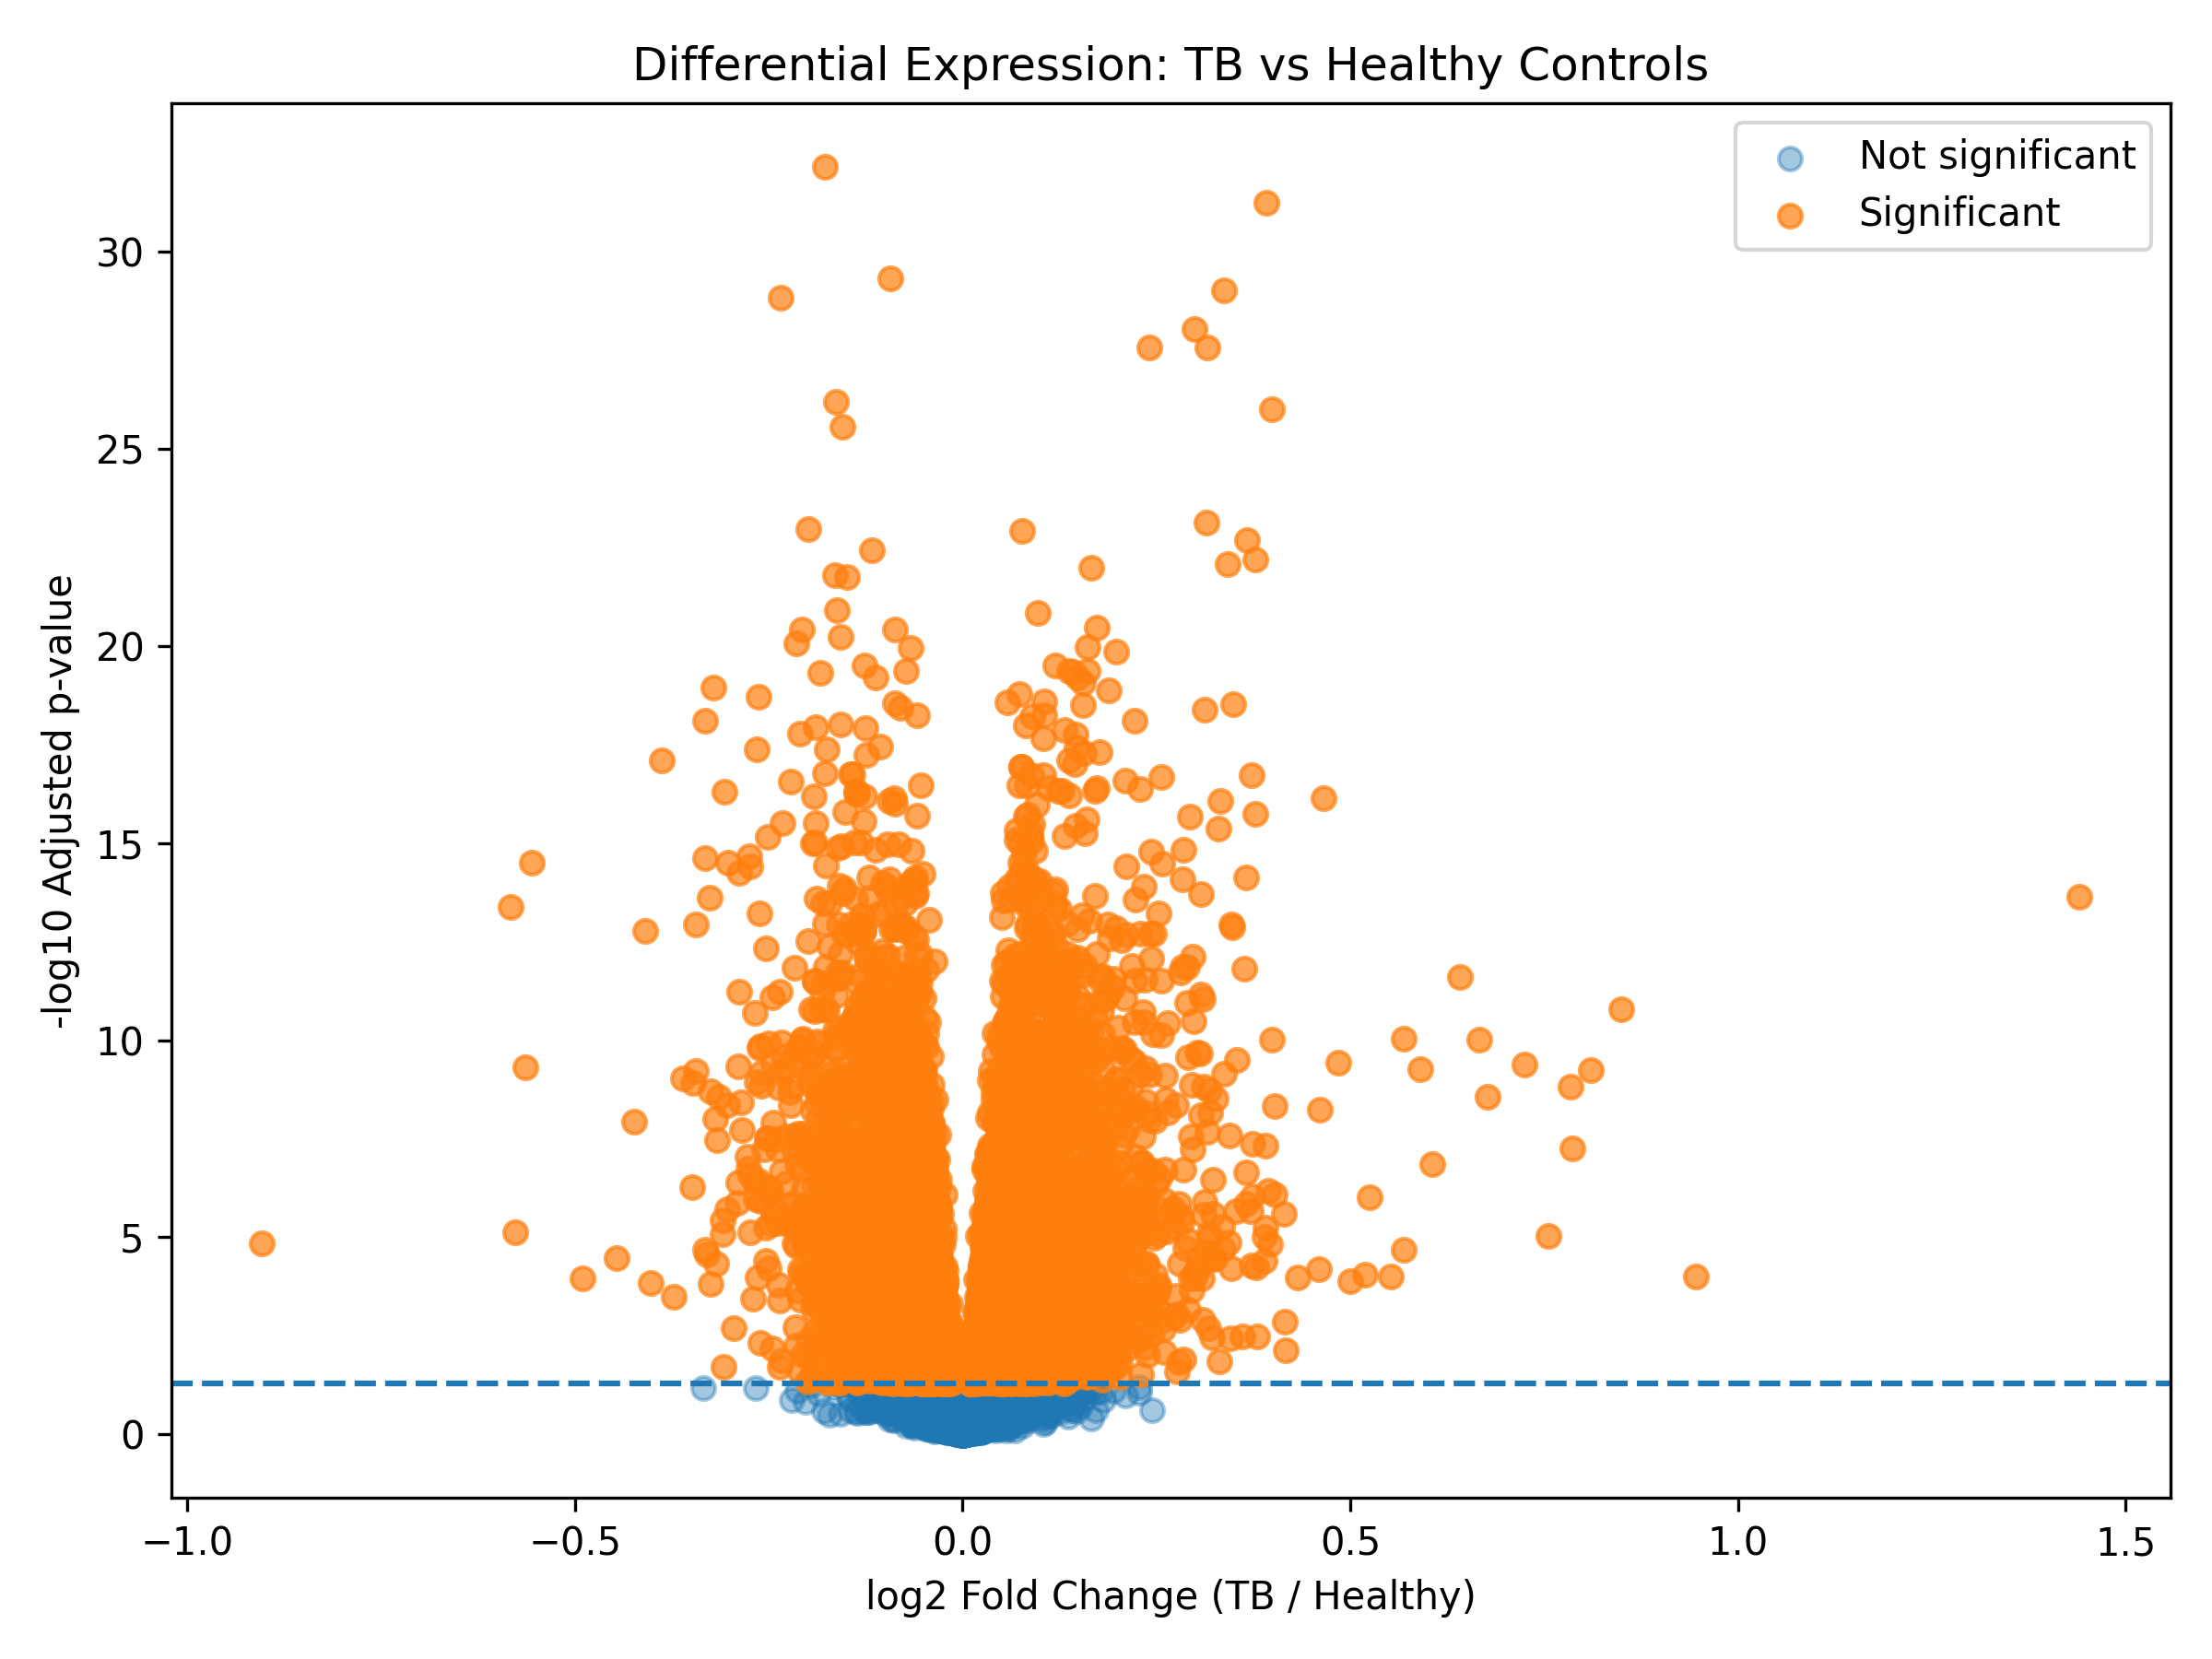
\includegraphics[scale=0.5]{volcano_plot.png}
		\caption{Volcano plot of differential expression results.}
		\label{fig:volcano}
	\end{figure}
	
	The table below lists the top 50 differentially expressed genes, including their log2 fold change, group means, $p$-value, adjusted $p$-value, and significance status. All 50 of the top differentially expressed genes were found to be significant.
	
	\begin{center}
		% TODO: insert table from results/top_50_differential_genes.csv
		\placeholder{[Table: Top 50 Differentially Expressed Genes --- results/top\_50\_differential\_genes.csv]}
	
	\end{center}
	
	\section{Heatmap of Significantly Differentially Expressed Genes}
	
	A heatmap was generated showing only the significantly differentially expressed genes (adjusted $p$-value $< 0.05$), with samples labeled by group (TB subjects vs.\ healthy controls) via a colored side bar. The heatmap shows that many genes have increased or decreased expression across the two groups, suggesting that TB infection is associated with broad changes across gene expression.
	
	\begin{figure}[h]
		\centering
		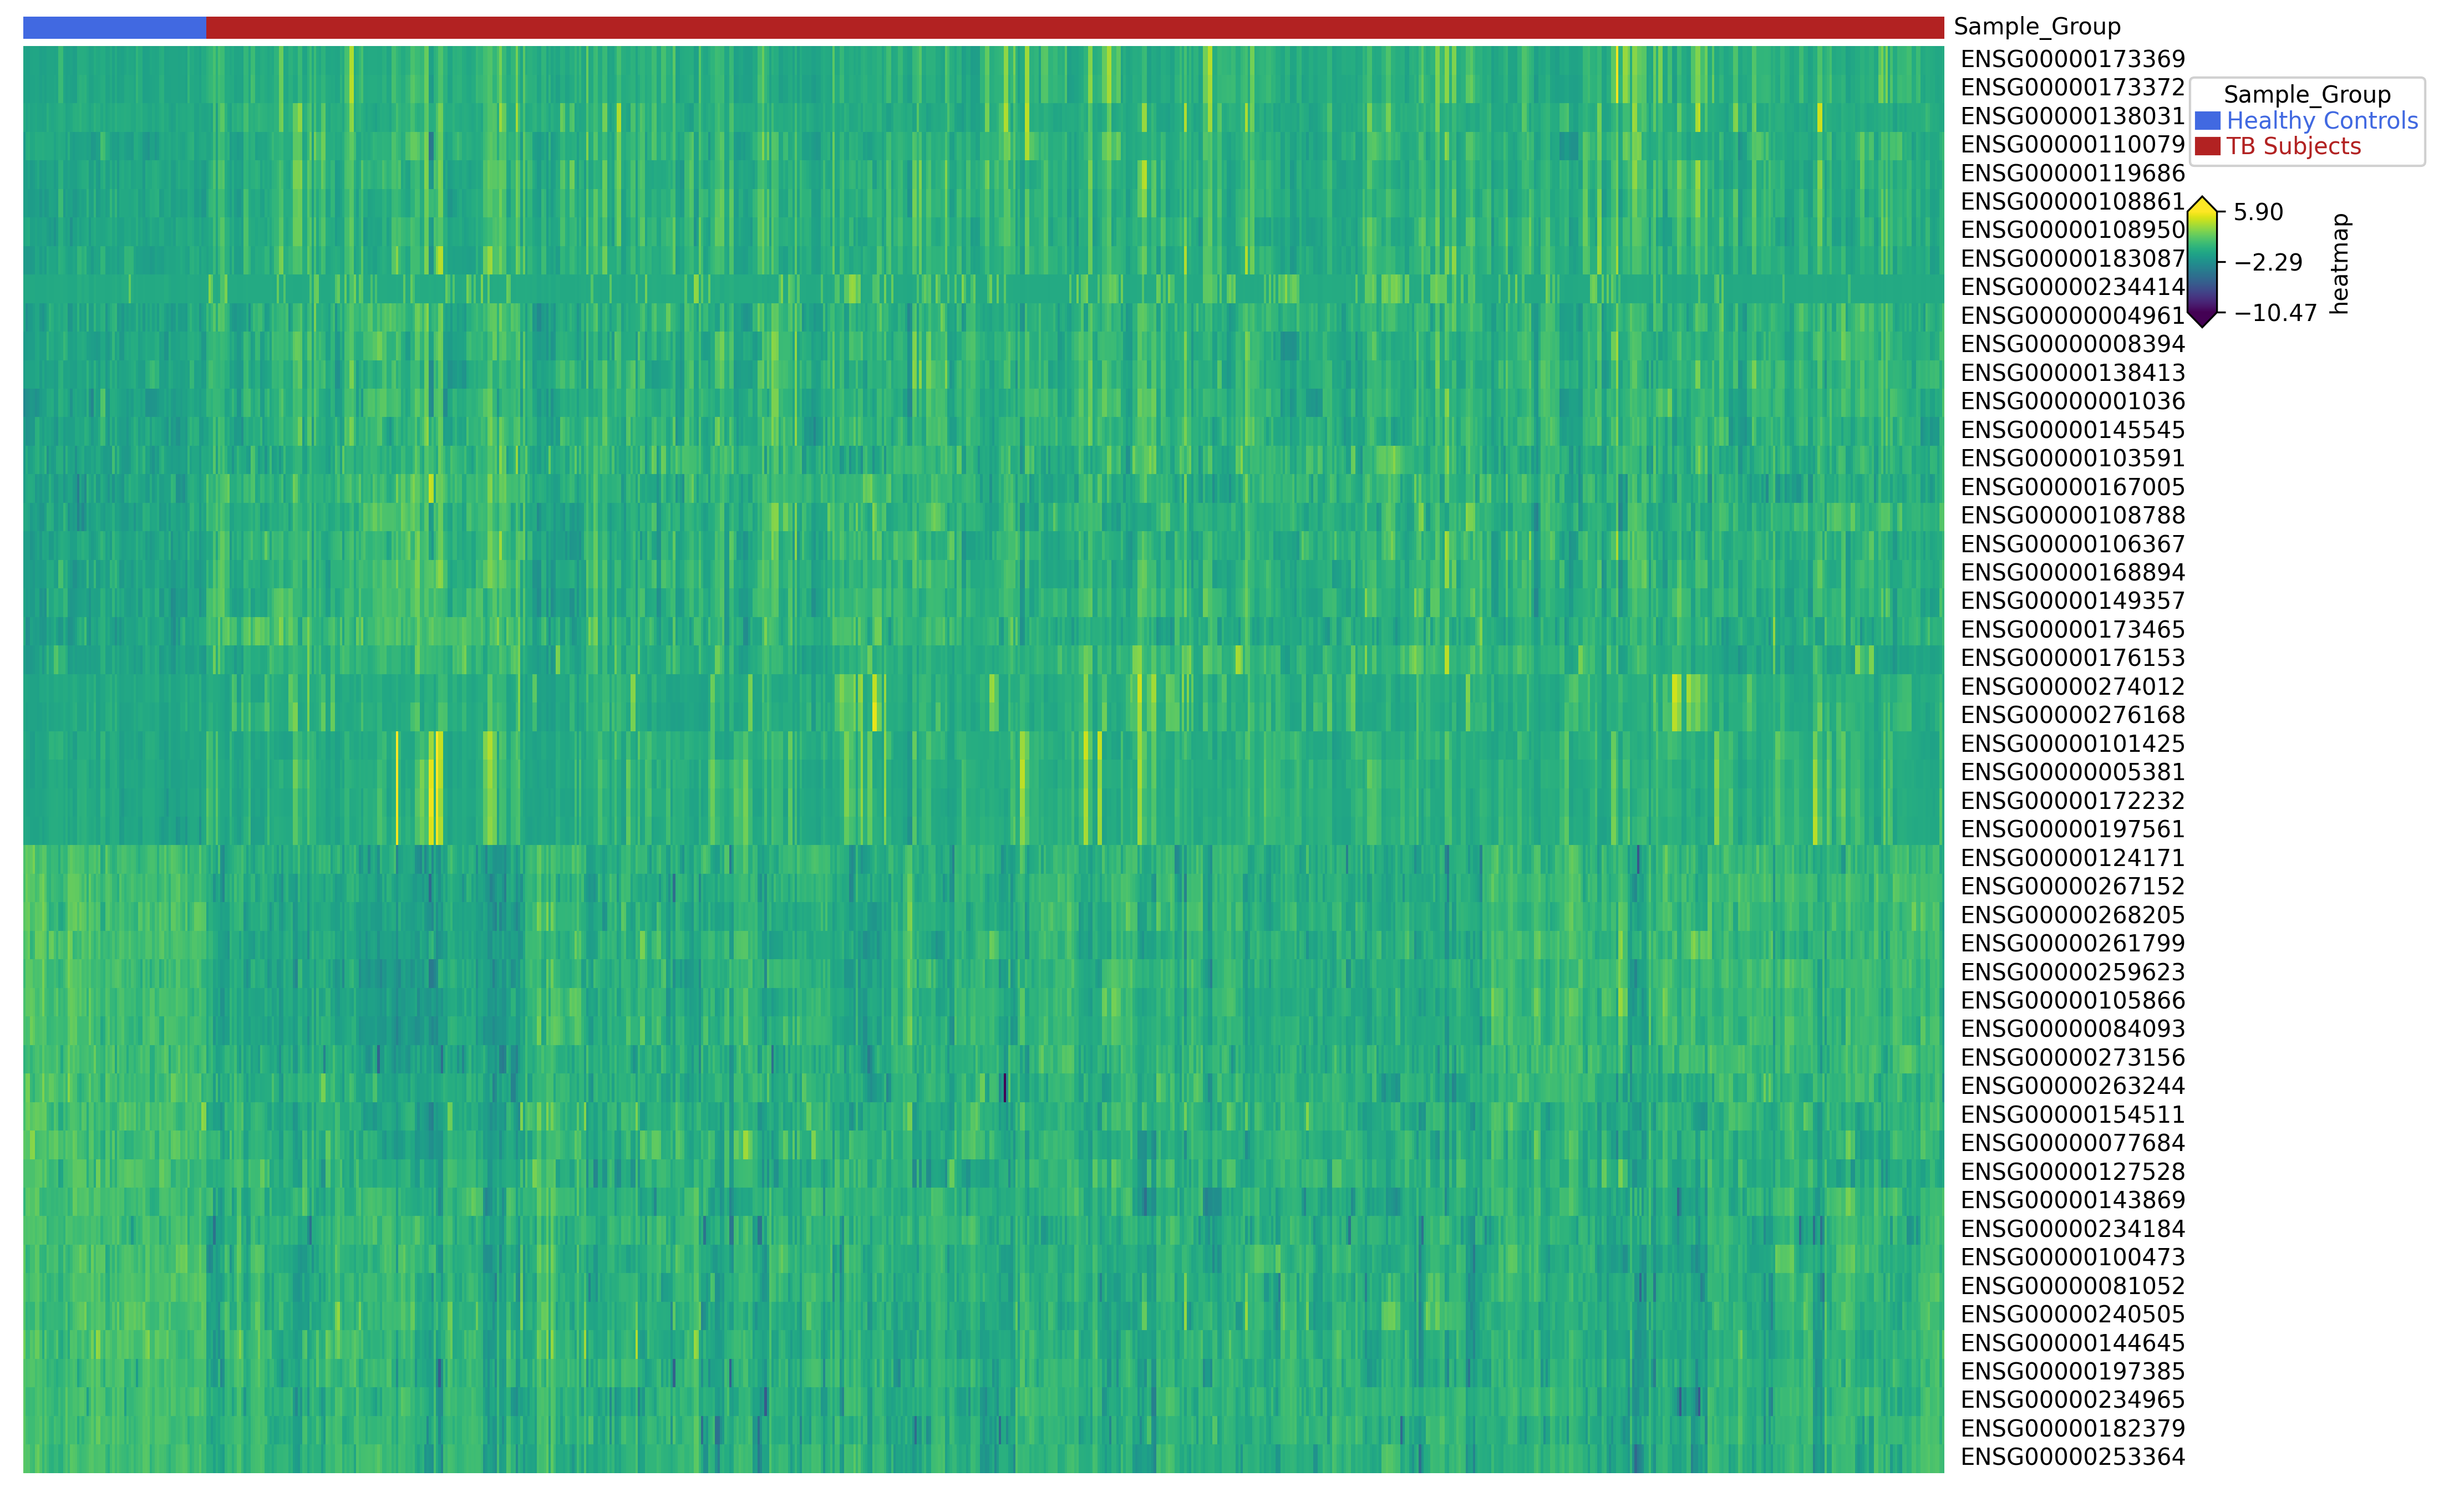
\includegraphics[scale=0.4]{DE_heatmap.png}
		\caption{Heatmap of significantly differentially expressed genes, annotated by sample group.}
		\label{fig:heatmap}
	\end{figure}
	
	\section{Gene Set Enrichment Analysis}
	
	Three enrichment methods were run across the team: clusterProfiler, gProfiler2, and the Wilcoxon rank-sum test. For clusterProfiler and gProfiler2, the significant gene list was defined using an adjusted $p$-value threshold of 0.05 combined with a $|\log_2 \text{FC}| \geq 0.3$ cutoff. Across these methods, results consistently pointed to genes with immune-related roles, including terms such as ``response to bacterium'' and ``regulation of innate immune response.''
	
	\subsection{clusterProfiler (GO: Biological Process)}
	
	% TODO: insert table from results/GO_BP_filtered_enrichment_clusterProfiler.csv
	\placeholder{[Table: clusterProfiler GO:BP enrichment results --- results/GO\_BP\_filtered\_enrichment\_clusterProfiler.csv]}
	
	\subsection{gProfiler2 (GO: Biological Process)}
	
	% TODO: insert table from results/filtered_enrichment_gprofiler_GO_BP.csv
	\placeholder{[Table: gProfiler2 GO:BP enrichment results --- results/filtered\_enrichment\_gprofiler\_GO\_BP.csv]}
	
	\subsection{Wilcoxon Rank-Sum Test}
	
	% TODO: insert table from results/rank_sum.csv
	\placeholder{[Table: Wilcoxon rank-sum enrichment results --- results/rank\_sum.csv]}
	
	\section{Joint Enrichment Table Across Methods}
	
	The results from the three enrichment methods were combined into a single joint table, with one row per unique GO term and columns indicating, for each method, whether the term was tested and whether it was found significant. Two summary columns record the number of methods that tested each term and the number of methods that found it significant. Of the terms tested, 24 genes/terms were found significant by all three methods, indicating a substantial degree of agreement across methods regarding genes with a significant impact on expression.
	
	\begin{center}
		% TODO: insert table from results/combined_enrichment.csv
		\placeholder{[Table: Combined Enrichment Results Across Methods --- results/combined\_enrichment.csv]}
	\end{center}
	
	\section{Top 10 Terms Enriched Across Methods}
	
	Using the joint table from Section 6, the top 10 terms most consistently enriched across the three methods were identified. This table shows a substantial number of terms that are enriched across all methods used in the analysis.
	
	\begin{center}
		% TODO: insert table from results/top_10_combined_enrichment.csv
		\placeholder{[Table: Top 10 Terms Enriched Across All Methods --- results/top\_10\_combined\_enrichment.csv]}
	\end{center}
	
\end{document}
